\section{Background}



\subsection{Basics of qLDPC codes}
Quantum low-density parity-check (qLDPC) codes are a class of quantum error-correcting codes defined by two sparse binary parity-check matrices $H_{X}$ and $H_{Z}$, which satisfy the commutation constraint $H_{X}H_{Z}^{T}=0$. These two matrices describe the stabilizer that detects errors, where $H_{X}$ corresponds to phase ($Z$) errors and $H_{Z}$ relates to bit-flip ($X$) errors, respectively. As shown in \autoref{fig:background} (a), the structure of qLDPC codes can be represented by a Tanner graph. It is a bipartite graph that connects data qubits to parity checks, where the edges stem from the non-zero entries in $H_{X}$ and $H_{Z}$. Measuring the parity check qubits will give the syndrome that encodes the error types and locations.

Unlike surface codes, where the decoding problem reduces to finding minimum-weight perfect matchings on a planar graph \cite{wu2023fusion,vittal2023astrea}, qLDPC codes generally induce a hypergraph structure due to the complex connectivity and the higher weight of stabilizers \cite{berlekamp2003inherent}. Each stabilizer can involve a logarithmic or constant number of qubits with non-local interactions, resulting in dense and irregular Tanner graphs. This hypergraph topology leads to an NP-hard decoding problem, where the ideal objective is to infer the most probable logical error given a syndrome \cite{iyer2015hardness}.

\begin{figure}[t]
\centerline{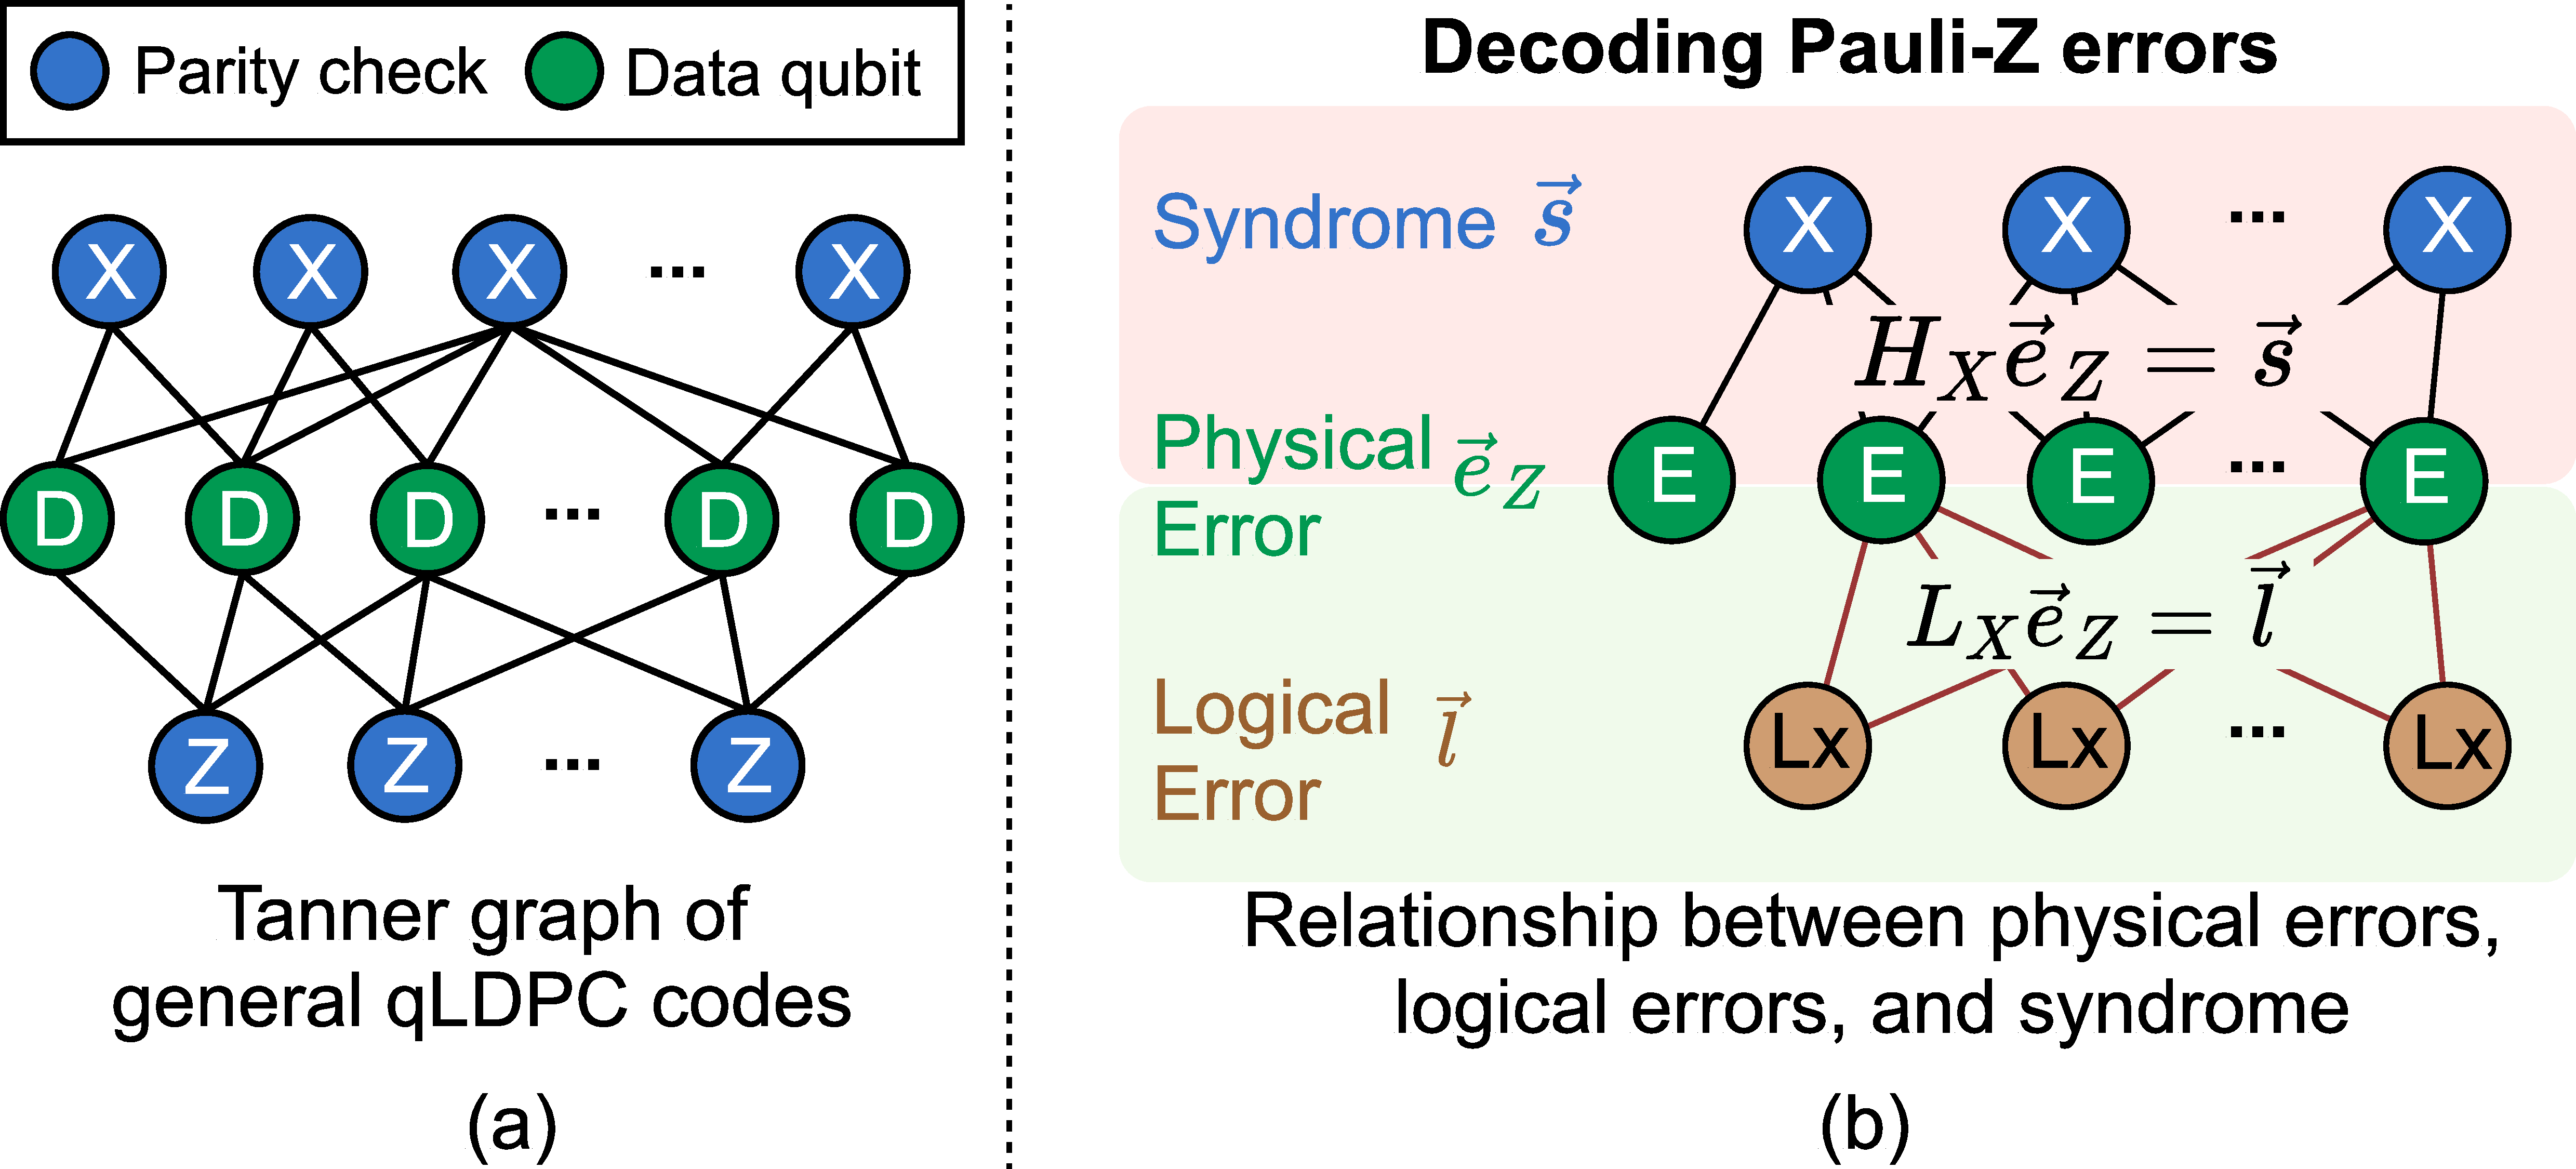
\includegraphics[width=1.0\columnwidth]{figures/background.pdf}}
\vspace{-0.4cm}
\caption{(a) Tanner graph of general qLDPC codes. (b) The relationship between physical errors,
logical errors, and syndrome. 
% (c) Illustration of BP and BP+OSD decoder. If BP fails to converge, it triggers the OSD part as post-processing.
} 
\vspace{-0.4cm}
\label{fig:background}
\end{figure}

\subsection{MLD Decoding}
% Decoding qLDPC codes requires a realistic noise model that reflects the behavior of actual quantum hardware. Simplified models (e.g., independent bit-flip) ignore the temporal and spatial correlations introduced by faulty quantum circuits. In contrast, the circuit-level depolarizing noise model accounts for errors during all elementary operations in the syndrome measurement circuit, including gate faults, qubit initialization and measurement errors, and idle decoherence. Each operation is assumed to fail independently with probability $p$, and upon failure, a uniformly random nontrivial Pauli error ($X$, $Y$, or $Z$) is applied to the affected qubit(s), consistent with a depolarizing channel. These errors may then propagate through the circuit, creating complex correlated error patterns that the decoder must properly handle.
Noise on the qLDPC codes circuit can be described as a physical error vector $\vec{e}$, where $e_j=1$ means an error occurs in the $j$-th position, while $e_j=0$ means no error in this position.
The physical errors can be decomposed into Pauli-X errors and Pauli-Z errors, which eventually cause the logical Pauli-X or Pauli-Z errors on logical qubits. Thus, the decoding objective of QLDPC is to infer the logical errors and correct the logical qubits. Since qLDPC codes belong to CSS codes, the Pauli-X and Pauli-Z errors can be decoded independently~\cite{bposd}. Without loss of generality, we focus on the decoding of Pauli-Z errors.

To detect the Pauli-Z errors $\vec{e}_Z$, measurements are applied on the X-type parity check qubits to give the syndrome vectors $\vec{s}$. 
As shown in \autoref{fig:background}~(b), the relationship between physical error $\vec{e}_Z$, logical error $\vec{l}$, and syndrome $\vec{s}$ can be expressed as
\begin{equation}\small\label{eq:decodingrelation}
    \begin{bmatrix} 
H_X \\ L_X
\end{bmatrix} \vec{e_Z} = \begin{bmatrix}
\vec{s} \\ \vec{l}
\end{bmatrix} \mod 2 \;.
\end{equation}
Here, $H_X$ is the parity check matrix, where each row is an X-stabilizer. $L_X$ is the logical check matrix, where each row is an X logical operator. 
% \autoref{fig:ablation_study}~(b) also shows the decoding relationship of Pauli-X errors and the commutation relationship between decoding Pauli-X and Pauli-Z errors.

% To decode under a circuit-level depolarizing noise model, a check matrix $H$ needs to be constructed, which maps circuit faults to measured syndromes across multiple rounds. \autoref{fig:background} (b) illustrates the syndrome measurement circuit of Bivariate Bicycle (BB) codes \cite{bbcode}, where parity checks interact with data qubits through CNOT gates and are measured to extract syndromes. Errors on CNOT gates, parity checks, or data qubits can propagate and affect the measured outcomes. For CSS-type qLDPC codes, $X$ and $Z$ errors can be decoded separately, allowing the construction of two independent decoding matrices $H_x$ and $H_z$. By unrolling the circuit over $d$ consecutive rounds, each column of $H_x$ or $H_z$ represents a fault event at a specific space-time location, and each row corresponds to a syndrome bit at a given round. As the number of measurement rounds increases, the decoding matrix grows vertically (more syndrome bits) and horizontally (more fault events), forming a temporally extended representation of the full decoding problem.



% \subsection{MLD decoding}

The maximum likelihood decoding (MLD) for qLDPC codes centers on finding the most 
likely logical error \( \vec{l}^* \) given an observed syndrome \( \vec{s} \), following \eqref{eq:decodingrelation}.
Here, we use Pauli-Z errors $\vec{e}_Z=\{e_1,e_2,\cdots,e_j,\cdots\}$ for illustration, where each error \( e_j \in \{0,1\} \) has physical error probability \( p_j \). The goal is to maximize the logical probability $P(\vec{l}|\vec{s})$ under a given syndrome $\vec{s}$,
\begin{equation}\small
\vec{l}^* = \arg\max_{\vec{l}} P(\vec{l}|\vec{s}).
\label{eq:logicalsyndrome}
\end{equation}
Here, the logical probability $P(\vec{l}|\vec{s})$ is calculated by accumulating all physical errors $\vec{e}_Z$ that belong to the logical error $\vec{l}$ and match the syndrome $\vec{s}$,
\begin{equation}\small \label{eq:logicalprobcons}
    P(\vec{l}|\vec{s}) = \sum_{\{\vec{e}_Z \mid 
H_X \vec{e}_Z = \vec{s}, L_X\vec{e}_Z  =\vec{l} \}} P(\vec{e}_Z) 
\end{equation}

\begin{equation}\small
P(\vec{e}_Z) = e^{-\sum_{j=1}^n 2w_j e_j}, \quad w_j = \ln \left( (1 - p_j)/p_j \right) /2 \label{eq:errorrate}
\end{equation}
where \( P(\vec{e}_Z)  \) is the physical error probability and $p_j$ is the phyiscal probability of occuring $j$-th error, \ie, $e_j=1$. $w_j$ is called error weight of $j$-th error.
After dedecting the moskly logical errors $\vec{l}^*$, the detected logical operator for error correction is,
\begin{equation} \small
    \hat{L} = H_{\text{des}}^T \vec{s} \oplus L_X^T \vec{l}^* \label{eq:recovererror}
\end{equation}
where $H_{\text{des}}$ is the matrix with each row a Z-destabilizer. 
% Since \eqref{eq:recovererror} is a deterministic process, the goal of maximum likelihood is to find the most likely logical errors in \eqref{eq:logicalsyndrome}.

% MWD decoders aim to identify the most probable physical error consistent with the observed syndrome. This formulation offers relatively low computational complexity, which makes these decoders practical for near-term implementations. However, it also inherently limits their decoding accuracy. As illustrated in the red bar of \autoref{fig:motivation}~(a), MWD focuses on recovering the most likely physical error, whereas the true objective of quantum error correction is to recover the most probable logical state (i.e., to identify the most likely logical coset), shown in the green region. Because qLDPC codes exhibit high \textit{quantum degeneracy}, multiple distinct physical errors can correspond to the same logical error. Consequently, the most likely physical error may reside in an incorrect logical coset, leading to logical failures even when the physical correction appears optimal \cite{gnd,cao2023qecgpt}. Therefore, while MWD decoders offer efficiency, their accuracy remains fundamentally suboptimal.

% For computational efficiency, we express this as:
% \[\small
% P(\vec{e}_Z) = e^{-\sum_{j=1}^n 2w_j e_j}, \quad w_j = \ln \left( (1 - p_j)/p_j \right) /2
% \]

% \subsection{BP and BP+OSD Decoder}
% The most widely used decoders for qLDPC codes are Belief Propagation (BP) \cite{bp} and Belief Propagation with Ordered Statistics Decoding (BP+OSD) \cite{bposd}, as shown in \autoref{fig:background}~(c).
% BP is an iterative probabilistic decoding algorithm that operates on the Tanner graph of the code, where messages representing error probabilities are exchanged between variable nodes (data qubits) and check nodes (parity checks). Through successive iterations, BP updates these messages based on the syndrome and the graph’s connectivity, gradually refining the posterior probabilities of qubit errors. However, in quantum codes, the presence of quantum degeneracy, where multiple distinct error patterns produce the same syndrome, can cause BP to converge to an incorrect solution.

% To address this limitation, the OSD technique is often integrated with BP as a post-process, forming the BP+OSD decoder. In this hybrid approach, BP is first used to estimate the error probabilities of data qubits. Then, OSD reorders the columns of the parity-check matrix according to these probabilities and applies Gaussian elimination to extract a set of linearly independent columns, transforming the matrix into an invertible form. This allows the decoder to directly compute an error pattern consistent with the syndrome by solving a linear system. By leveraging the probability information provided by BP, OSD corrects for the failures caused by quantum degeneracy and significantly improves decoding accuracy.